\documentclass[UserManual.tex]{subfiles}
\begin{document}
\begin{sloppypar}

\section{Plotting Programs}\label{sec:figs}

\subsection{Overview}
The {\it Smooth Emulator} distribution includes three plotting programs, all based on PYTHON's MATPLOTLIB. The first program allows the User to visualize the accuracy of the emulator by comparing emulator predictions to full-model calculations at random points not used to train the emulator. The other two plotting programs illustrate the results of the MCMC constraint of model-parameter space.

\subsection{Preparing the Data Files for the Plots}
The plotting programs are contained the {\tt  \$\{MY\_ANALYSIS\}/figs/} directory. Within that directory is a file, {\tt directions.pdf}, which is a copy of this chapter. The three plotting programs are located in the three subdirectories, {\tt figs/YvsY}, {\tt figs/posterior} and {\tt figs/resolvingpower}. Before running the plotting programs, one must first create several data files and move them to the {\tt figs/figdata} directory. This directory will hold all data required to make the plots. Thus, none of the plotting functionality depends on the location of the {\tt figs/} directory, as long as the {\tt figdata/} directory is a subdirectory of the same directory as {\tt YvsY/}, {\tt posterior/} and {\tt resolvingpower/}.

The first data file is {\tt figdata/prior\_info.txt}. This file provides the plotting programs with the names of the model parameters, both the short-hand names and the \LaTeX name. To create the file, one can first copy the file of the same name from the {\tt smooth\_data/Info/} directory, then edit. The file should have three columns describing the model parameters:
\vspace*{-8pt}{\tt
\begin{Verbatim}
 parameter_name_1 prior_type_1 axis_name_1
 parameter_name_2 prior_type_2 axis_name_2 
 .
\end{Verbatim}
}\vspace*{-8pt}
The first column lists the ascii names, which are the same as those in {\tt smooth\_data/Options/prior\_info.txt}. For example, the model parameter might be named {\tt initial\_temperature}. The second column is the prior type, either {\tt uniform} or {\tt gaussian}. The first two columns are unchanged from the original file. The third column, which is new, provides the strings for labeling the axes in the plots. For example, this might be {\tt \$T\_0\$}. These are not purely \LaTeX formats, but are those used by MATPLOTLIB, which differ from standard \LaTeX because some of the backslash commands require double backslashes, e.g. \Verb{\r} needs to be \Verb{\\r}. The names in the last column are arbitrary and are only used to label axes. All elements of the file must be strings of characters without spaces.

The second file, {\tt observable\_info.txt}, is also created by initially copying the file of the same name in the {\tt smooth\_data/Info/}. The new file, {\tt figdata/observable\_info.txt} must then be edited. As the name implies it provides the names of the various observables to be plotted. The file format is:
\vspace*{-8pt}{\tt
\begin{Verbatim}
observable_name_0  axis_name_0
observable_name_1  axis_name_1
 .
 \end{Verbatim}
}\vspace*{-8pt}
The first column is exactly the same as the original file, and the last column provides the {\LaTeX}-like labels for the axes.

If the User wishes to plot the comparison between emulator predictions and actual full-model values, they must move the directory {\tt smooth\_data/FullModelTestingRuns/} to the {\tt figs/figdata} directory.
\vspace*{-8pt}{\tt
\begin{Verbatim}
% cp -r $\{MY_ANALYSIS\}/smooth_data/FullModelTestingRuns $\{MY_ANALYSIS\}/figs/figdata/
}\vspace*{-8pt}
In the tutorial, that directory, and its files, are created by running  the {\tt fakefullmodel} program, which calculated the full-model values at a set of randomly-chosen points. Within that directory are separate files providing the comparison between the full-model and the emulator predictions. The files are named {\tt YvsY\_[observable-name].txt}. Here {\tt [observable-name]} must match the ascii names from {\tt figdata/observable\_info.txt}. If the calculation compares observables at $n$ points, the file format for each of the $N_{\rm obs}$ files is:
\vspace*{-8pt}{\tt
\begin{Verbatim}
 Y1_full   Y1_emulator emulator_uncertainty_1  accuracy_1
 Y2_full   Y2_emulator emulator_uncertainty_2  accuracy_2
   .
 Yn_full   Yn_emulator emulator_uncertainty_n  accuracy_n
\end{Verbatim}
}\vspace*{-8pt}
The first and second columns give the full-model and emulator values for each of the randomly chosen points in model-parameter space. The third column lists the emulator's prediction of its uncertainty at those points. The final column lists the deviation between the full-model and emulator values scaled by the uncertainty. Only the first three columns are used by the plotting program.

If the User wishes to visualize the posterior by sampling the MCMC trace or if they wish to plot the resolving power extracted from the MCMC trace data, they should move the following files to the {figs/figdata/} directory.
\vspace*{-8pt}{\tt
\begin{Verbatim}
% cp $\{MY_ANALYSIS\}/smooth_data/MCMC/trace_theta.txt $\{MY_ANALYSIS\}/figs/figdata/
% cp $\{MY_ANALYSIS\}/smooth_data/MCMC/ResolvingPower.txt $\{MY_ANALYSIS\}/figs/figdata/
}\vspace*{-8pt}

\subsection{Running {\tt YvsY.py} to Compare Emulator Predictions to the Full-Model}
To perform this comparison, one must enter the {\tt figs/YvsY/} directory and run the PYTHON script:
\vspace*{-8pt}{\tt
\begin{Verbatim}[commandchars=\\\{\}]
{\tt \$\{MY\_ANALYSIS}/figs/YvsY% \textcolor{darkred}{python3 YvsY.py}
--- Observables ---
iY= 0   observable_name_0
iY= 1   observable_name_1
iY= 2   observable_name_2
iY= 3   observable_name_3
 .
Enter iY to designate observable: \textcolor{darkred}{XXX}
XXX of 100  points within 1 sigma
\end{Verbatim}
}\vspace*{-8pt}
As shown above, the script prompts the User to name which observable is being considered. The User should enter $n=${\tt `0',`1',`2'}$\cdots$ to denote the observable in the provided order. If the User enters `3', emulator predictions for the observable {\tt observable\_name\_3} will be evaluated. A plot should appear:
\begin{figure}
\centerline{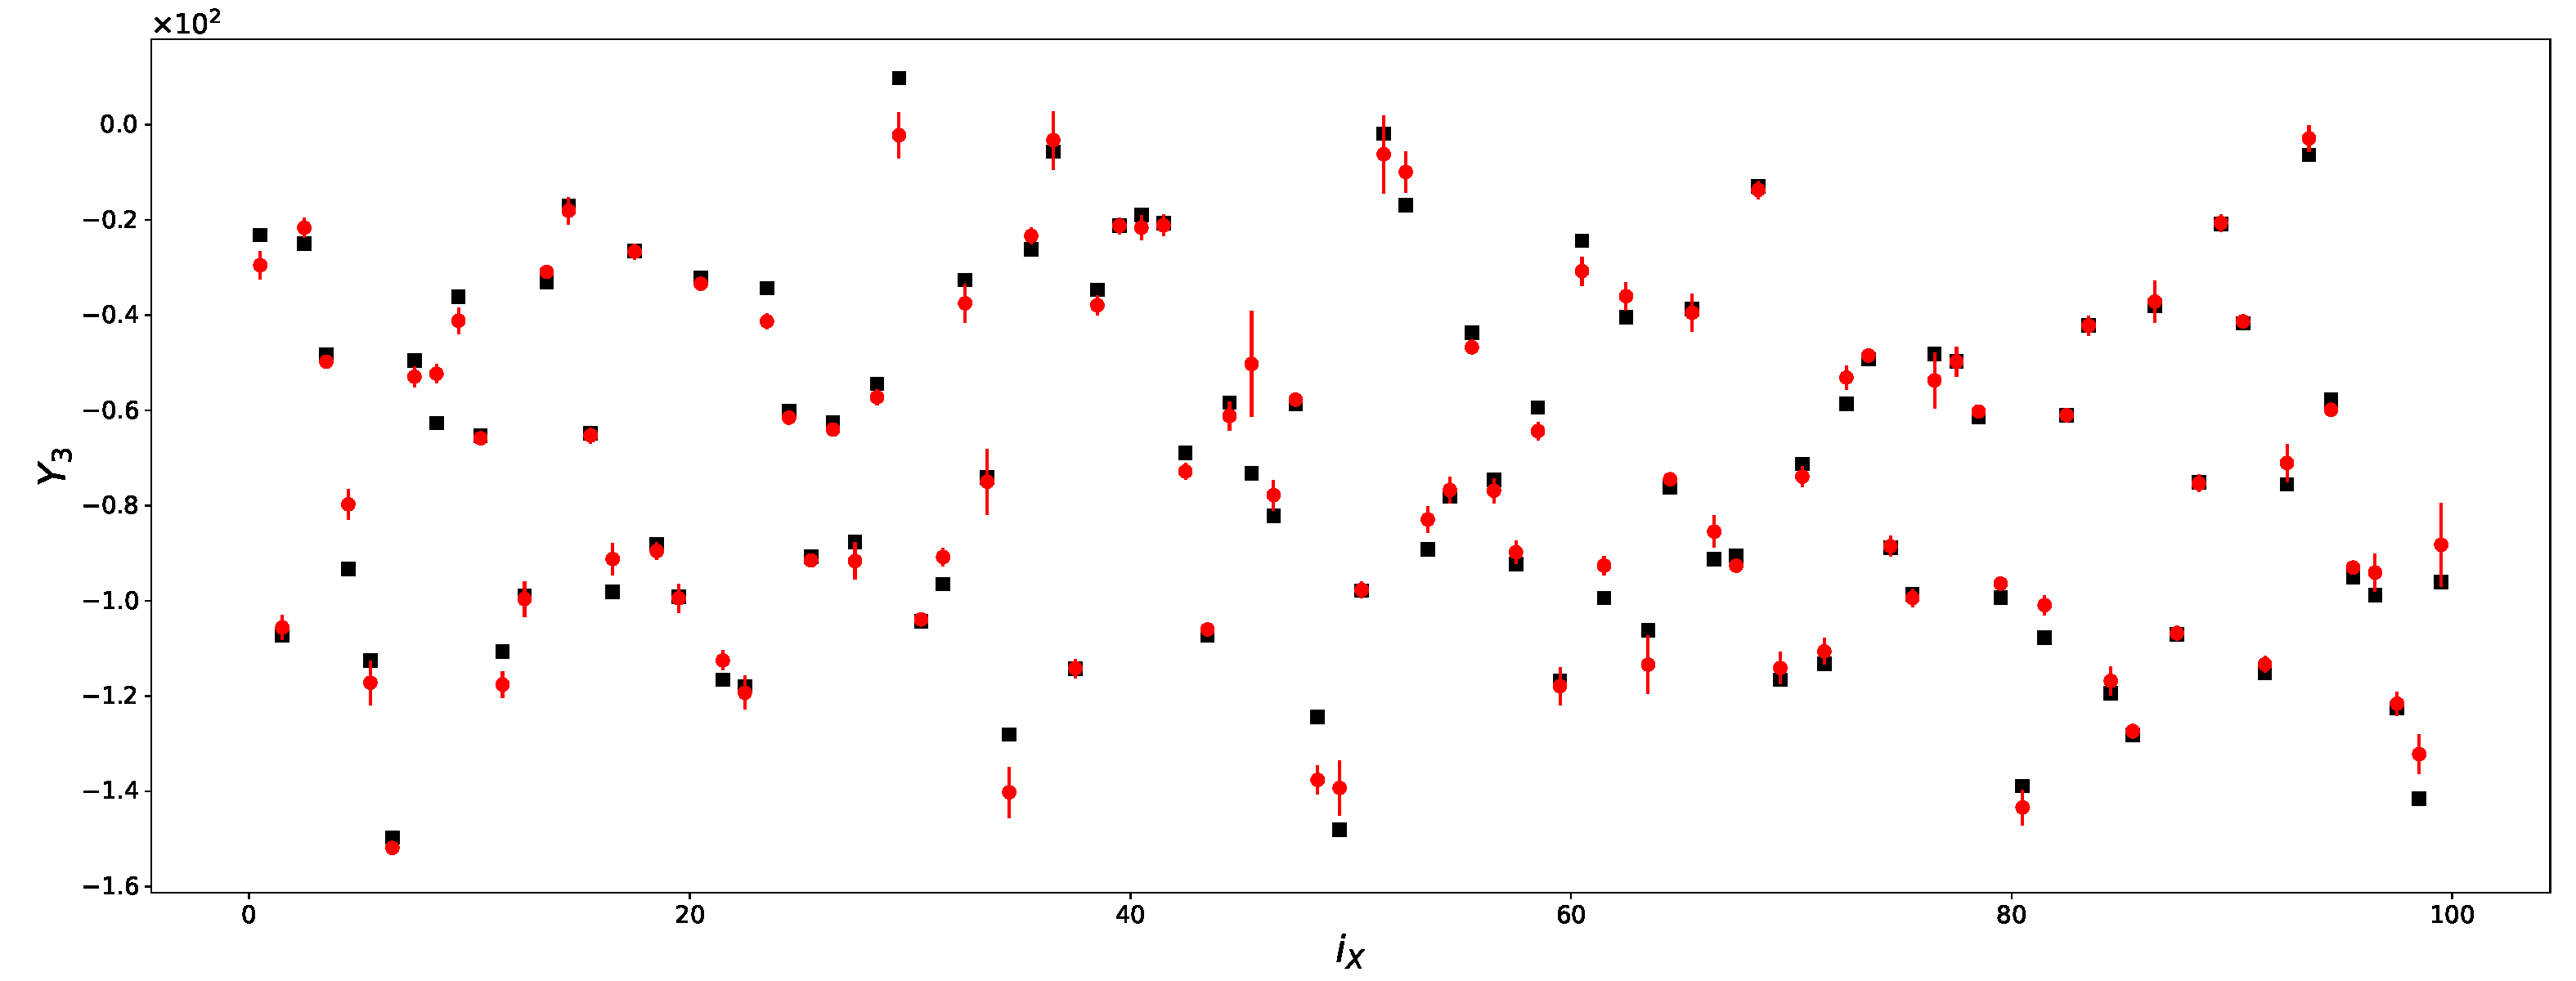
\includegraphics[width=\textwidth]{figs/YvsY_tutorial}}
\caption{\label{fig:YvsY_directions}
For the case plotted here 100 model-parameter points, noted in the plot by $i_x$, were evaluated. The black squares show the full-model values and the red points show the emulator predictions along with their error. When the program finishes the plot is also prints out how many of the comparisons were within one unit of the emulator uncertainty, denoted by {\tt XXX} in the output above. If the emulator were to accurately state its uncertainty, 68.3\% of the points would be within one $\sigma$.}
\end{figure} 

If the User wishes to view the PDF file of the plots, rather than the python version, they can go into the file and comment out the {\tt plt.show} line, then uncomment the lines calling the system commands:
\vspace*{-8pt}{\tt
\begin{Verbatim}
 .
# if you have Mac OS and want to see pdf file, comment out previous two lines and uncomment line below
#os.system("open -a Preview "+outputfilename);
# if you have Linux and want to see pdf file, comment out previous two lines and uncomment line below
#os.system("okular "+outputfilename+"&");
 .
\end{Verbatim}
}\vspace*{-8pt}
It is likely the User will wish to alter the plots for their purpose. Hopefully, the PYTHON script is sufficiently straight-forward to make such edits without too much difficulty.

\subsection{Running {\tt posterior.py} to View the Posterior Constraints of the Model-Parameter Space}
To view the posterior distribution, enter the {\tt figs/posterior/} directory and run the PYTHON script:
\vspace*{-8pt}{\tt
\begin{Verbatim}[commandchars=\\\{\}]
{\tt \$\{MY\_ANALYSIS}/figs/YvsY% \textcolor{darkred}{python3 posterior.py}
Number of points in trace = XXX
\end{Verbatim}
}\vspace*{-8pt}
The script reads the MCMC trace data and creates a plot, an example of which is shown here.\\
\begin{figure}[h]
\centerline{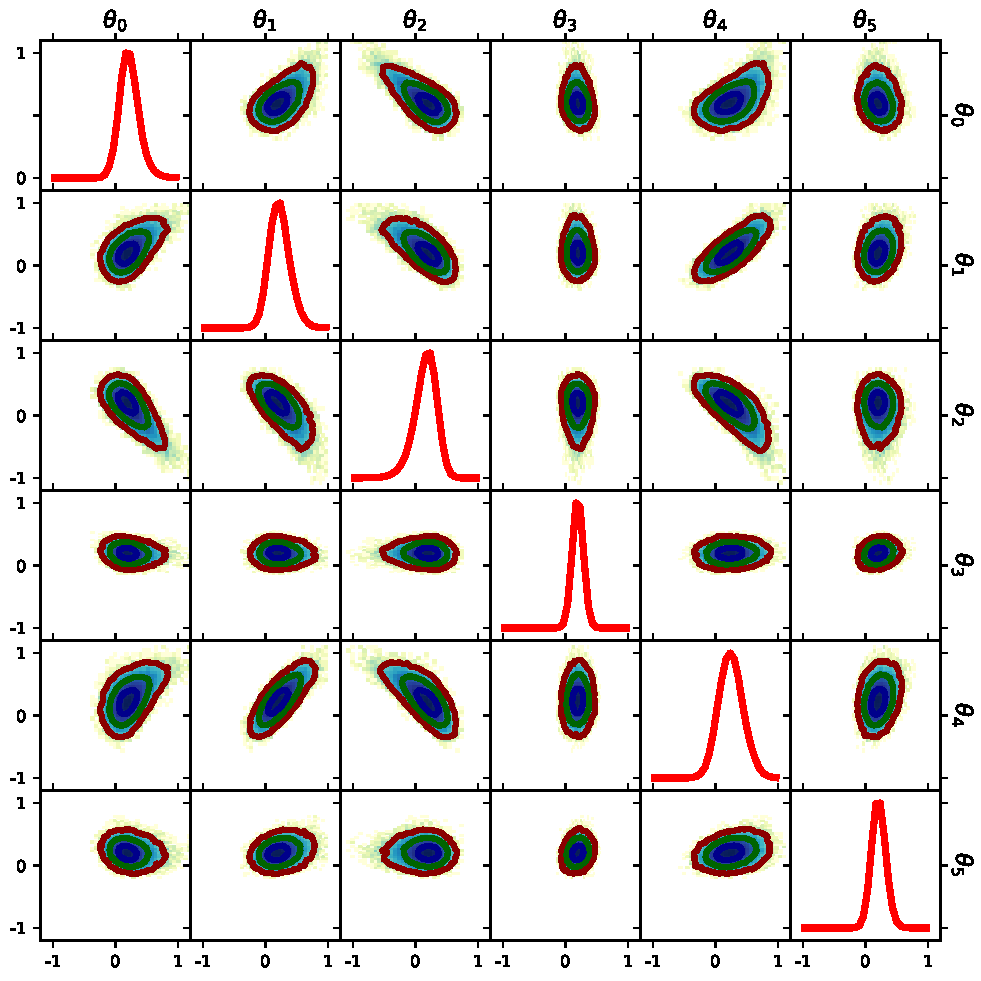
\includegraphics[width=0.8\textwidth]{figs/posterior_tutorial}}
\caption{\label{fig:posterior_directions}
As was the case before one can edit the lines near the bottom of the file to display the PDF file.
}
\end{figure} 

For this example, the ``experimental'' data was generated by running the model with each model parameter set to $\theta_i=0.2$. One can see that the procedure was rather successful in finding the correct values, which serves as a self-consistency check.

The User should note that the scaled coordinates, $\vec{\theta}$, are used instead of the real coordinates. This choice was made simply because the unscaled coordinates might have complicated bounds, which might be difficult to list given the small sub-panels. The User should also note that the posterior includes the constraints of the prior. Hence, if some parameter had a Gaussian prior, and was not at all further constrained by the analysis, it would still appear as a non-uniform distribution in the plot.

The User needs to choose what subset of the observables they wish to consider in the plot. This is done by editing the Python script, {\tt figs/posterior/posterior.py}. One must edit the line
\vspace*{-8pt}{\tt
\begin{Verbatim}[commandchars=\\\{\}]
 .
ParsToPlot=[0,1,2,3,4,5]
 .
\end{Verbatim}
}\vspace*{-8pt}
If there were 6 observables, this would then consider all of them. Otherwise, one should adjust the list accordingly.

\subsection{Running {\tt RP.py} to View the Resolving Power}
\begin{figure}[hb]
\begin{minipage}{0.6\textwidth}
One measure of an observable's resolving power with respect to constraining a specific model parameter is defined as the amount the posterior average of the constrained model parameter, $\langle\langle X\_i\rangle\rangle$, is likely to change given a change of the observable, $\langle\langle Y\_i\rangle\rangle$, scaled by the variance of $Y\_i$ in the prior. The MCMC analysis program created a file {\tt smooth\_data/MCMC/ResolvingPower.txt}, which the User has moved to the {\tt figs/figdata/} directory. By entering the {\tt figs/resolvingpower/} directory and running the PYTHON script, one creates a figure showing the resolving power,
\vspace*{-8pt}{\tt
\begin{Verbatim}[commandchars=\\\{\}]
{\tt \$\{MY\_ANALYSIS}/figs/YvsY% \textcolor{darkred}{python3 RP.py}
 NPars= XXX NObs= XXX
\end{Verbatim}
}\vspace*{-8pt}

\vspace*{1.1in}

\caption{\label{RP_directions}
An example of the resolving power. Positive/negative values mean that the extracted model parameters are increased/reduced if the observable grows. If the magnitude of the bar is large, the extracted model parameter is strongly sensitive to the observable.}
\end{minipage}
\begin{minipage}{0.4\textwidth}
\centerline{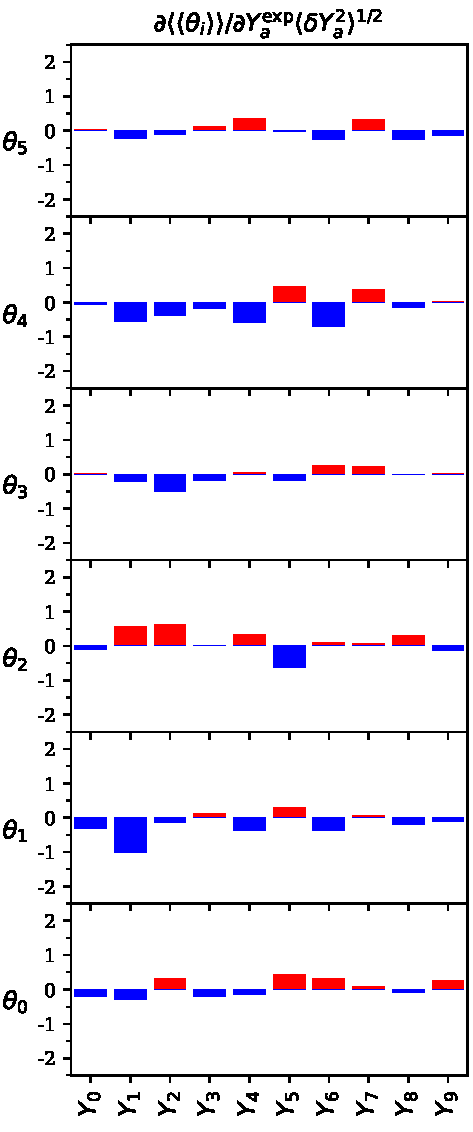
\includegraphics[width=0.8\textwidth]{figs/RP_tutorial.pdf}}
\end{minipage}
\end{figure}

\end{sloppypar}
\end{document}